\chapter{Огляд Open Data Cube та супутникових даних}
\section{Open Data Cube}
Open Data Cube [6, 11] - це спеціалізований програмний продукт з відкритим кодом, для керування та проведення аналізу геопросторових супутникових даних.

Даний продукт має потужні можливості, щоб проводити різні дослідження та завантажувати необхідну інформацію, що надходять від супутників.

Основні переваги системи Data Cube:

Каталог великих геопросторових обсягів даних.

API на основі Python для високопродуктивних запитів.

Надає вченим та іншим користувачам легку можливість виконувати дослідницький аналіз даних.

Дозволяє масштабовану обробку даних континенту, що зберігається.

Можна відстежувати походження всіх даних, що містяться, щоб забезпечити контроль якості та оновлення.

Мета ODC - збільшити роль супутникових даних наданням відкритого та доступного дослідницького інструменту та сприяти розвитку сфери аналізу даних супутників. Це рішення має на меті підтримати ключові цілі, що включають в себе полегшення використання даних та підтримувати глобальні пріоритетні міжнародні програми. ODC повинен створити "бренд", якому користувачі можуть довіряти, і він повинен сприяти позитивному користувальницькому досвіду. Це має стати можливим завдяки розробці спільноти ODC з відкритим кодом, яка активно займається розробкою, ділиться алгоритмами та надає підтримку один одному для вирішення проблем.

Як це рішення дозволяє задовольнити попит багатьох світових користувачів з обмеженими ресурсами? Масштабованість - одна з ключових проблем, з якою стикається ODC. Хоча початкові зусилля привели лише до декількох національних масштабів впровадження Data Cube (наприклад, Австралія, Колумбія, Швейцарія), Є багато інших країн та глобальних організацій, що мають високий інтерес до ODC. Завдяки взаємодії з зацікавленими організаціями та поточними користувачами, очікується, що кількість ODC збільшиться і спільнота ODC процвітатиме з розширенням своїх можливостей.

Ядро ODC служить прошарком між супутниковими постачальниками даних та додатками. Існує набір інструментів з відкритим кодом, щоб допомогти вченим проводити дослідження, використовуючи дані, якими керує ODC. Популярні інструменти, що використовуються у спільноті, яка використовує ODC Core як основу, включають:

Командний рядок: інструмент, який використовують програмісти / розробники для взаємодії з ODC.

Відкритий ODC: Візуальний та інтерактивний веб-додаток, який дозволяє користувачам досліджувати свій інвентар наявних даних.

ODC статистика: Оптимізований засіб проведення розширеного аналізу в системі ODC. Цей інструмент орієнтований на вчених.

Веб-інтерфейс ODC: веб-додаток, який дозволяє розробникам інтерактивно демонструвати та візуалізувати вихід алгоритмів.

Jupyter Notebook: Такі файли дають інтерактивну можливість візуалізувати аналізовані дані.

Веб-сервіси відкритого геопросторового консорціуму: адаптери, які можуть підключати додатки non-ODC до ODC.

Усі вищеописані інструменти формують користувацьку структуру управління Open Data Cube.

У роботі був використаний ODC, який керується Інститутом космічних досліджень НАН України та ДКА України.

Причина використання ODC

Причиною використання ODC у роботі стала розвиваюча спільнота, легкість та швидкість завантаження знімків супутника родини Sentinel-2 і прикладні програми обробки з використанням мови програмування Python \cite{ref10}, за допомогою яких відбувалось композитування, візуалізація. Але найбільша перевага ODC є масштабованість даних, що означає можливість завантажувати і опрацьовувати як завгодно великі території.

\section{Супутник Sentinel-2}
У даній роботі використовувалися дані космічної місії Sentinel-2 [1, 2], що дають композити у багатьох каналах.

Композит \cite{ref15} - це сукупність каналів, що використовуються для візуалізації зображенння.

Перший супутник Sentinel-2A даної місії був запущений у 2015 р, а другий Sentinel-2B у 2016 р. Розрізнення знімків, що дають апарати -- 10, 20 та 60 м, знімають у 12 каналах (Таблиця 2. 1). Частота зйомки на рівні екватора - раз в п'ять днів, у середніх широтах - раз у два-три дні.

Таким чином, сімейство супутників Sentinel -2 надає достатньо багато корисної інформації та даних, щоб робити наукове дослідження у сфері аналізу супутникових даних та моніторингу земного покриву Землі.

\chapterConclusion
Отже, Open Data Cube - це безкоштовний програмний продукт та спільнота, що розвиває можливості аналізу супутникових даних і не тільки. Супутникові дані, що надає сервіс COAH є 4 канальними композитами RGBN та відповідною маскою хмарності.

\chapter{Уточнення маски хмар}
\section{Маска хмарності}
Разом з композитами cервіс COAH [1, 2, 6] надає також і маску хмарності. Вона є масивом із розмірністю, що співпадає з розмірністю самого знімку, де кожен піксель має значення від 0 до 11 (Таблиця 3. 1). Це певний класифікатор, де цифра позначає область знімка, наприклад хмари, рослинність чи перисті хмари. Відповідно ми можемо одержати інформацію про кожний піксель композиту, а саме чи є він захмарений чи ні.

Відповідно для вилучення хмар було побудовано бінарну маску, яка складалася з 2,3,8 та 9 значень оригінальної маски. Даний масив потрібний для накладання на композит, щоб класифікувати піксель як такий чи він захмарений чи ні.

\section{Недоліки маски хмар від COAH}
На жаль, дані що дає copernicus hub, не є ідеальними, саме це стосується і маски хмар. Після написання алгоритму було проведено перші його тестування, результат був неякісним.

Було проведено дослідження чому це відбувається, і виявилось, що не до всіх знімків класифікатор для маски надається в тому ж самому розрізнення що і відповідний йому 4 канальний композит. Дана проблема потребувала вирішення як і для покращення оригінальної маски так і для алгоритму вилучення хмар.

\begin{figure}[H]\centering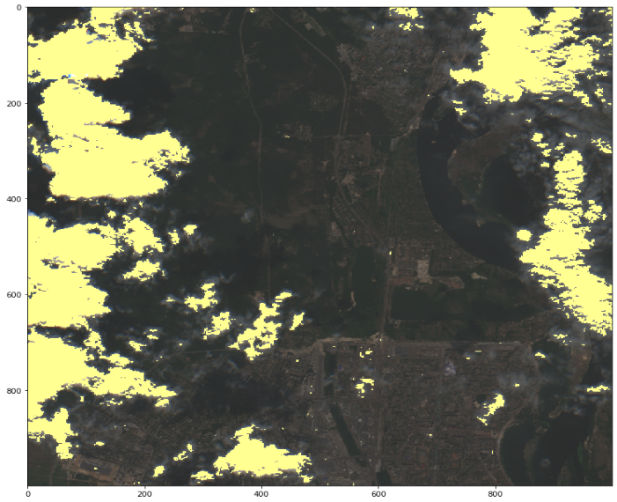
\includegraphics[width=0.82\textwidth]{images/image5.png}\caption{Ілюстрація з вихідної роботи (image5)}\label{fig:image5}\end{figure}
На завантажених файлах супутникових знімків із розрізненням 10 м була виявлена маска із розрізненням 20, що й приводило до проблеми

того, що реальні хмари на композиті не покривались класифікатором (Рисунок 3.1).

\section{Розширення маски хмар}
Для уточнення маски хмар був використаний алгоритм Dilation.

Розширення (Dilation) [3,4] - один з двох основних операторів математичної морфології, інший - ерозія. Зазвичай він застосовується до двійкових зображень, але є версії, які працюють на зображеннях grayscale зображень. Основний ефект оператора на бінарне зображення полягає в поступовому збільшенні меж областей пікселів переднього плану. Таким чином, ділянки пікселів переднього плану збільшуються в розмірі, тоді як отвори в цих регіонах стають меншими.

Як це працює, нехай у нас є деяка множина множина , яка потребує розширення, та певний структурний елемент , тоді - проекція , що переміщена на зрушення . Розширення (Формула 3.1), це множина всіх зрушень, що задовольняють умові:

\begin{equation}\label{eq:dilation}A\oplus B=\{s\mid B_s\cap A\ne\varnothing\}.\end{equation}
(3.1)

Якщо зображення це f(x), а структурний елемент b(x), тоді розширення (Формула 3.2) f на b.

\begin{equation}\label{eq:dilation-function}(f\oplus b)(x)=\sup_{y\in E}\{f(y)+b(x-y)\}.\end{equation}
при використанні великих структурних елементів, то b(x) формується (Формула 3.3)

(3.3)

де B є підмножиною

в даному випадку розширення будується так (Формула 3.4):

( (3.4)

Сам процес розширення (Рисунок 3. 2) є не складним: нехай є певна множина, яка потребує збільшення або розширення, тоді існує ще одна множина, яка виступає у ролі структурного елемента. Тоді структурний елемент проходиться по межам розширюючої множини і збільшує її границі на заданий розмір. Таким чином, ми одержуємо множину, що має ту ж саму форму, що й оригінальна, але вже збільшена.

Розглянемо приклад застосування оператора розширення

у випадку супутникових даних, а саме окремого композиту та його маски.

З цього знімка (Рисунок 3. 3) був зроблений композит та взята його маска (Рисунок 3. 4). З маски було витягнуто окремі пікселі, що відповідають окремо за перисті хмари та самі хмари. Тобто взято \{10\} та \{2,3,8,9\} значення пікселів відповідно та розширено (Рисунок 3. 5) за допомогою оператора.

\begin{figure}[H]\centering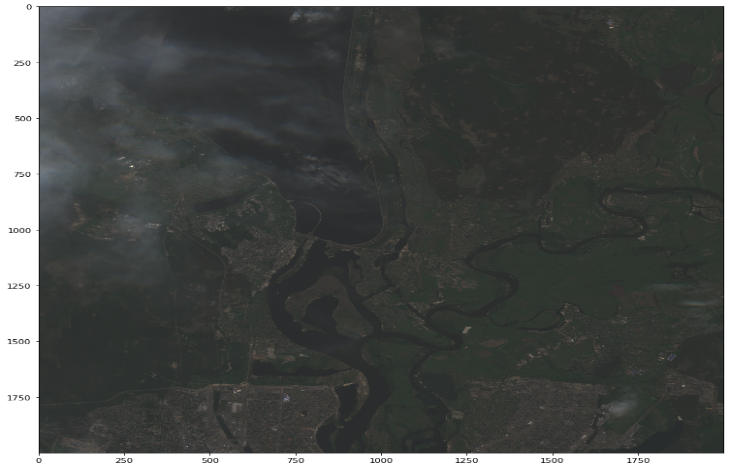
\includegraphics[width=0.82\textwidth]{images/image7.png}\caption{Ілюстрація з вихідної роботи (image7)}\label{fig:image7}\end{figure}
\begin{figure}[H]\centering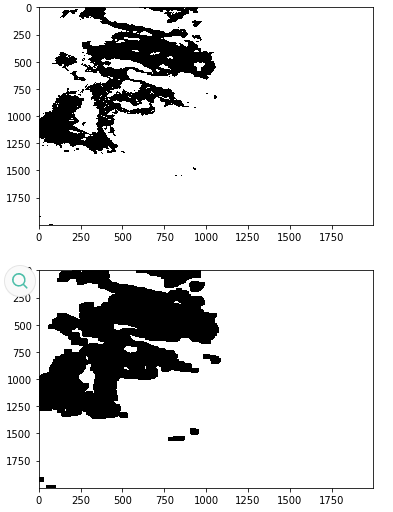
\includegraphics[width=0.82\textwidth]{images/image8.png}\caption{Ілюстрація з вихідної роботи (image8)}\label{fig:image8}\end{figure}
\begin{figure}[H]\centering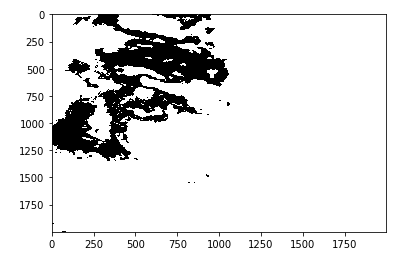
\includegraphics[width=0.82\textwidth]{images/image9.png}\caption{Ілюстрація з вихідної роботи (image9)}\label{fig:image9}\end{figure}
\chapterConclusion
Був зроблений огляд маски хмарності, що надається серсвісом COAH. Виявлено, що вона не покриваэ реальни хмар, тому було запропоновано вперше використати морфологічний оператор розширення, як спосіб уточнення маски хмарності. Наведений приклад застосуваня даного оператора на масці хмар.

\chapter{Алгоритм вилучення хмарних пікселів}
Для аналізу та тестуваня алгоритму брались дані за червень 2019 року Київської області. З ними був проведений глибокий аналіз на відповідність та можливість подальшої обробки, оскільки якщо в одній серії за місяць будуть знімки де хмарність складає більше 50\% то на виході алгоритму буде композит, в якого багато пікселів матимуть чорний колір.

Тобто постала проблема відбору даних, що більш-менш підходять під реалізацію методу. Також цей процес потрібно було повністю автоматизувати, оскільки не зручно власноруч шукати потрібні знімки.

Дана проблема була вирішена за допомогою саме застосування Open Data Cube. ODC надав змогу автоматично та швидко завантажувати дані просто увівши параметри часу, широти, висоти та супутника.

Було написано процедури, які давали відсоток хмарності, що покращило обробку і тим самим відкидались знімки за тей час де відсоток хмарності перевищував 35\%.

\section{Алгоритм}
Спочатку всі датасети, що були завантажені потрібно очистити від знімків, кожен канал яких мав значення nan, тобто це просто зображення чорного кольору.

Потім було прийнято рішення про сортування композитів по проценту хмарності, інія та неповних знімків. Даний функціонал був доданий в ODC. Неповний знімок, це такий самий по розмірності знімок, що і інші в датасеті, але не відображена вся територія. Таким чином відбирались такі дані де відсоток загальної хмарності був не більшим за 35-40 відсотків, оскільки, інакше вихідний знімок після роботи алгоритму буде з дефектами.

На вхід процедури (Додаток А), що прибирає хмари подається множина індексів часу та сам датасет, звідки ці знімки. Тут, вже ці знімки пройшли повний препроцесинг і готові для обробки. Дана процедура (Рисунок 4. 1) повинна повернути певну кількість композитів, які потім будуть оброблятися медіаною.

Для того щоб проводити вищенаведені операції з великим датасетом, у якого більше ніж два знімки, було розроблено декілька способів обробки. А саме, наступні.

Нехай в якості вхідного використовується датасет, в якому знімки проіндексовані наступним чином: [1,2,3,4,5,6....]. Тоді для побудови безхмарного композиту використано наступні методи комбінування знімків:

Кожний з кожним:

Даний алгоритм полягає у комбінуванні кожний з кожним, тобто [1.2],[2.1], але не сам з собою.

В результаті можна отримати якісне зображення, але з суттєвими затратами комп’ютерних ресурсів. На виході буде композитів, при вхідних знімків.

Почергова трійка

На вхід моделі подається почергова трійка, де перший знімок буде базовим

Приклад; [1,2,3], [2,3,4], [3,4,5]

Даний метод дає оптимальну якість і є більш ощадливим до обчислювальних ресурсів.

Було досліджено швидкодію (Рисунок 4. 2) кожного з описаних методів комбінування.

З урахуванням отриманих результатів експериментів має сенс в подальшому використовувати метод парами кожний з кожним при відносно малій кількості знімків і почерговою трійкою, якщо нас цікавить збереження обчислювальних ресурсів чи часу.

Вихідний знімок був побудований за допомогою метода кожний з кожним.

Для майбутнього покращення якості та швидкості опрацювання великих датасетів було розглянуто наступні методи комбінування знімків:

Кожний базовий

На вхід подаються списки виду [1,2,3,4,..], [2,1,3,4,..], [3,1,2,4,..],

Тобто завжди подається весь датасет, причому перший знімок є базовим, а на наступному кроці попередній базовий міняється місцями з наступним.

Пріоритетність

Спочатку робиться сортування знімків по хмарності у датасеті.

Нехай є впорядковані знімки [3,2,5,7,6,4,1], тоді 3-ій є базовим. Наступні ітерації будуть побудовані таким чином:

3,2,5,7,6,4

3,5,7,6,4

3,7,6,4

3,4

Цей метод буде працювати виключно якщо базовий знімок з дуже малим відсотком хмарності.

Для досягнення найкращої якості вихідного композиту потрібно брати знімки, які є максимально близькими за часом зйомки. Це забезпечить менший перепад у відтінках пікселів. Таким чином після комбінування знімків і заміни захмарених пікселів, маємо кінцевий масив наступного вигляду.

\begin{figure}[H]\centering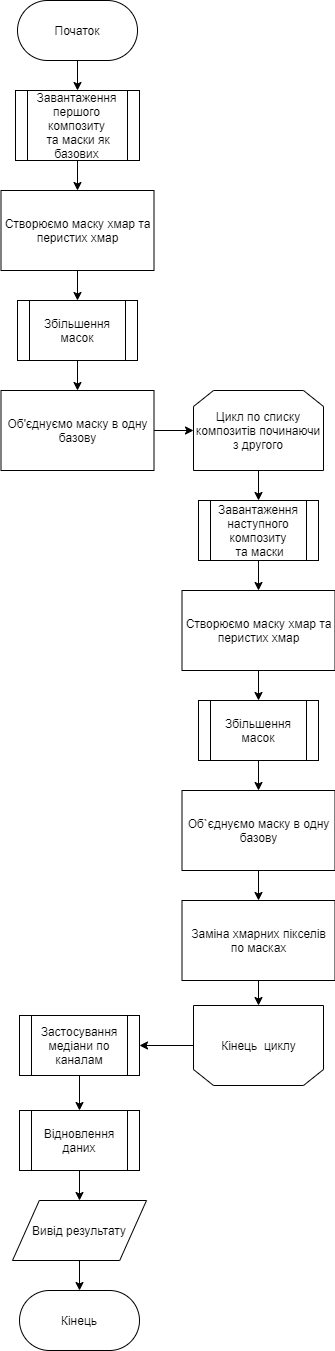
\includegraphics[width=0.82\textwidth]{images/image10.png}\caption{Ілюстрація з вихідної роботи (image10)}\label{fig:image10}\end{figure}
\begin{figure}[H]\centering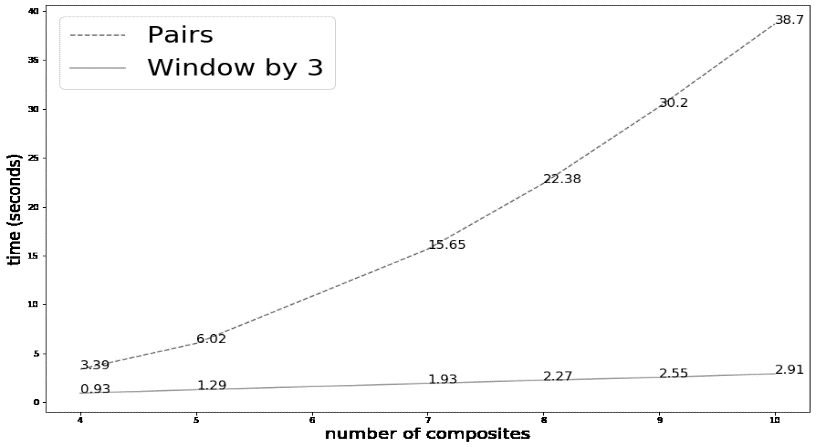
\includegraphics[width=0.82\textwidth]{images/image11.png}\caption{Ілюстрація з вихідної роботи (image11)}\label{fig:image11}\end{figure}
\section{Медіана по каналам}
Щоб отримати цілий єдиний знімок з мінімальним по кількості захмарених пікселів, було використано медіану \cite{ref5}. Дана процедура на вхід отримує кілька знімків (Рисунок 4. 3) та проходить по кожному каналу кожного знімка, тим самим формуючи єдине число, а саме піксель окремого каналу. Причому дана медіана не чіпає пікселі, які не містять ніякої інформації (NODATA).

Таким чином створюється масив (4,x,y) (Рисунок 4. 4), де x, y - розмірність вхідних знімків, 4- це канали Red, Green, Blue та Nir.

\begin{figure}[H]\centering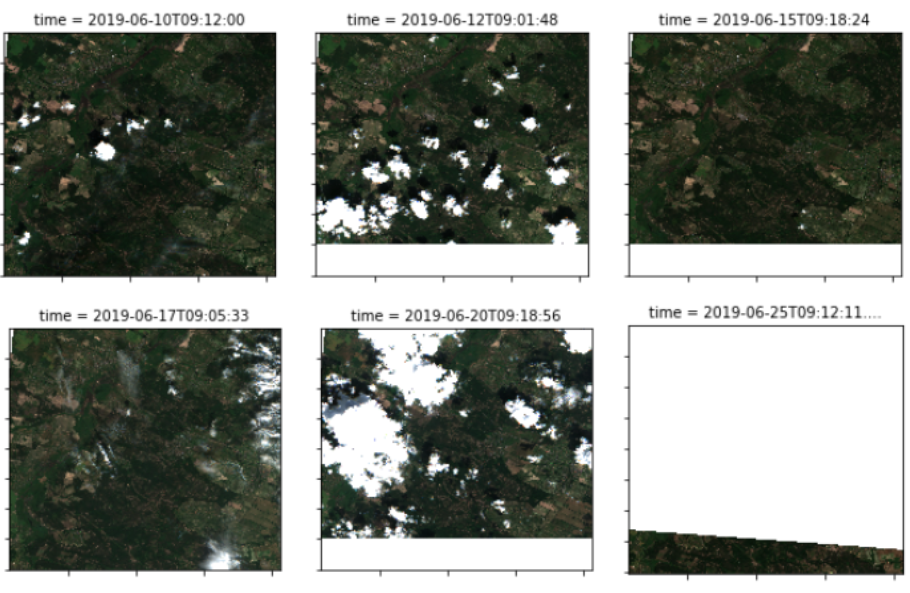
\includegraphics[width=0.82\textwidth]{images/image12.png}\caption{Ілюстрація з вихідної роботи (image12)}\label{fig:image12}\end{figure}
\begin{figure}[H]\centering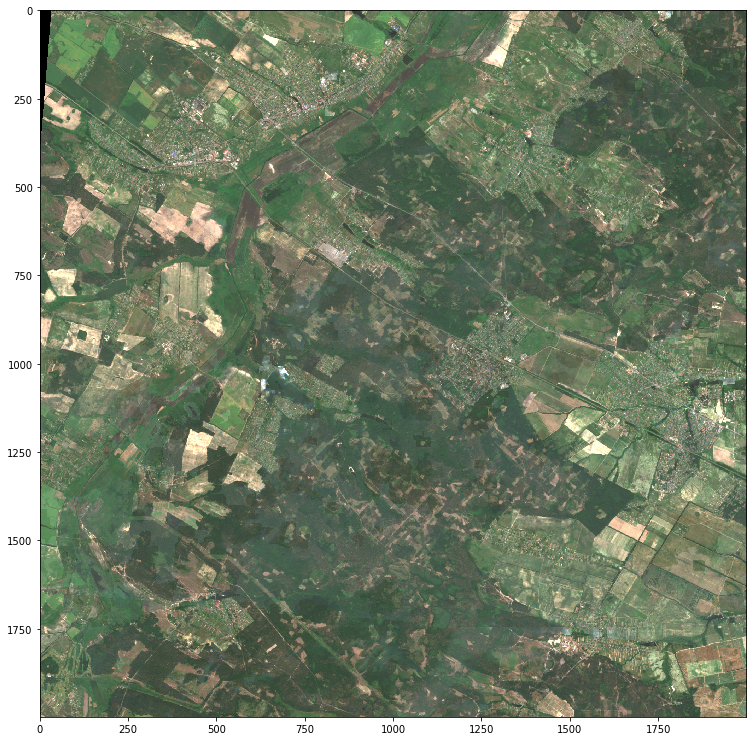
\includegraphics[width=0.82\textwidth]{images/image13.png}\caption{Ілюстрація з вихідної роботи (image13)}\label{fig:image13}\end{figure}
\chapterConclusion
Був побудований алгоритм вилучення захмарених пікселів, використана медіана по каналам, як спосіб одержання єдиного знімку, запропоновано методи кобінування знімків коли композитів більше двох. Таким чином на виході отримується максимально безхмарий знімок з 4-ма каналами RGBN.

\chapter{Модель відновлення супутникових даних}
Часто в супутникових даних зустрічаються ситуації, коли в датасеті є неповні знімки (Рисунок 5. 1).

\begin{figure}[H]\centering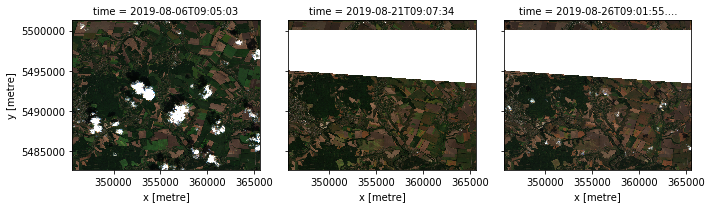
\includegraphics[width=0.82\textwidth]{images/image14.png}\caption{Ілюстрація з вихідної роботи (image14)}\label{fig:image14}\end{figure}
Нажаль, саме через такі випадки в безхмарному результуючому знімку можна помітити, що на деяких частинах зображення (Рисунок 5. 2) можна побачити різницю між колірними просторами, а саме на одному з регіонів може бути більше зелені або навпаки менше, що буде одразу помітно на цілому зображенні.

Тому постає задача у вирішенні проблеми. Необхідно розглянути алгоритми мета яких - переведення колірного простору між зображеннями.

\begin{figure}[H]\centering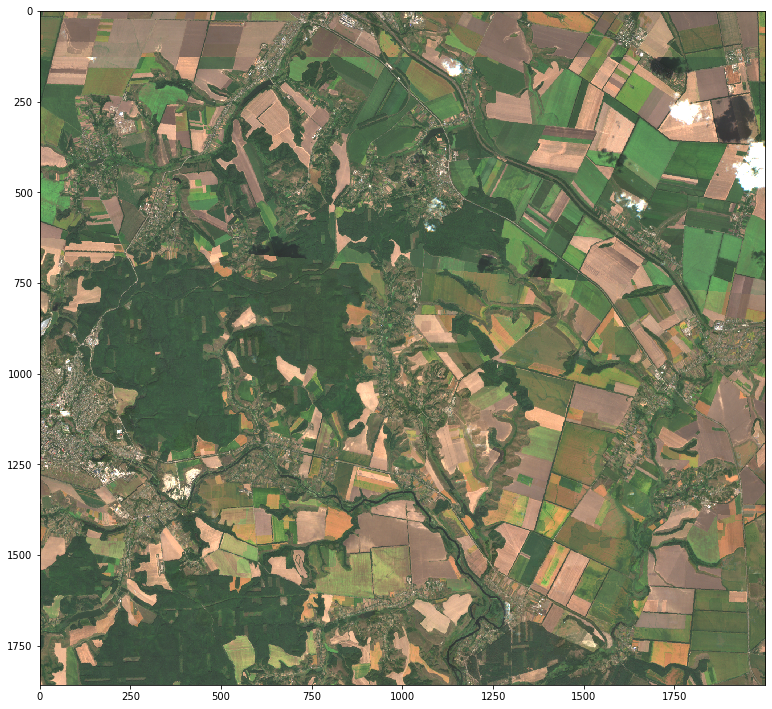
\includegraphics[width=0.82\textwidth]{images/image15.png}\caption{Ілюстрація з вихідної роботи (image15)}\label{fig:image15}\end{figure}
\section{Color Transfer between Images}
Дан Рудерман та інші спеціалісти. розробили кольоровий простір, який називається lαβ, що мінімізує кореляцію між каналами для багатьох природних сцен. Даний простір був зроблений на аналізі того як сприймає та обробляє вхідну інформацію зорова система людини природні сцени. Автори представили новий формат lαβ беручи за основу зорову систему людини.

Між осями у просторі lαβ є вирази, що дозволяють нам використовувати різні дії в різних каналах, при чому не переживаючи, що не з’являться дефекти на зображенні. Плюс - цей колірний простір логарифмічний, що значить нормальне масштабування.

Даний алгоритм \cite{ref8} досі не розглядався у контексті роботи із супутниковими знімками. Тому є необхідність зробити певний аналіз щодо того чи слід його використовувати між сусідніми регіонами, оскільки до цього його застосовували тільки для звичайних RGB зображень.

Було запрограмовано вищеописаний алгоритм та виявлено такі факти:

Не було знайдено методу, що переводить Geotiff знімок у формат LAB.

Проблема полягає в тому, що оригінальний алгоритм перенесення кольору загалом працює із зображеннями з малим масштабом, а саме наприклад значення [0 - 255]. У знімках формату Geotiff діапазон набагато більший [0 - 10 000].

Метод не може забезпечити правильну відповідність територій.

Тут мається на увазі, що якщо на зображенні на яке ми хочемо накласти новий колірний простір є регіон наприклад лісів чи полів, то після обробки ті ж самі регіони мають і залишитись лісами чи полем.

Провівши аналіз алгоритму перенесення колірного простору було прийнято рішення щодо застосування методів машинного навчання, адже саме завдяки ним можна одержати правильне зображення де у відповідності зі знімком з якого беруть колір на знімку до якого його застосували будуть максимально наближені регіони по свої притаманності, тобто якщо було озеленене поле воно стане більш сухим і світлим, якщо такі були наявні у знімку з якого брали стиль.

Коли мова йде про обробку супутникових зображень і щоб на виході отримувати не класифікатор, а значення пікселів, то загалом використовують регресійні методи \cite{ref9} машинного навчання.

До найбільш придатних алгоритмів які вміють працювати зі знімками відносять лінійну, поліноміальну, баєсову регресії, регресію в методі опорних векторів та відомий багатошаровий перцептрон і алгоритм випадкового лісу. Вважаючи доцільним їх застосування у даній роботі, потрібно зробити їхній огляд.

\section{Лінійна регресія}
У математичній статистиці лінійна регресія \cite{ref7} --- це метод побудови залежності між змінною y та векторною залежною змінною X.

При використанні даного алгоритму машинного навчання взаємозв'язок між даними будується, використовуючи лінійні функції, при чому невідомі параметри функції отримуються за вхідними даними. Так само як і інші регресійні моделі лінійна регресія повертає розподіл умовної ймовірності y в залежності від X.

Для знаходження параметрів лінійної регресії у загальному випадку використовується метод найменших квадратів (МНК). Також існує можливість використання методу найменших квадратів для нелінійних моделей.

Якщо говорити мовою формул (Формула 5.1):

\begin{equation}\label{eq:linear}y=f(x,b)+\varepsilon.\end{equation}
де - параметри моделі, - випадкова похибка моделі.

називається лінійною регресією, якщо подається у вигляді (Формула 5.2):

\begin{equation}\label{eq:linear-model}f(x,b)=\sum_{j=1}^{k}b_jx_j=x^Tb.\end{equation}
- параметри регресії, - регресори, - кількість факторів у моделі

Також виділяють і так звану множинну регресію, що подається у вигляді (Формула 5.3):

(5.3)

\section{Баєсова регресія}
У даному алгоритмі \cite{ref7} машинного навчання лежить в основі вищеописана лінійна регресія. Тут так само визначена регресійна модель (Формула 5.4):

\begin{equation}\label{eq:bayes}y_i=\alpha+\beta x_i+\varepsilon_i.\end{equation}
Тут - незалежні та нормально розподілені випадкові величини з нульовим середнім та дисперсією .

Визначимо функцію максимальної правдоподібності (Формула 5.5):

(5.5)

Для того, щоб знайти розв’язок (Формула 5.6) за допомогою відомого методу найменших квадратів використовують псевдообернення Мура-Пенроуза :

\begin{equation}\label{eq:least-squares}\beta=(X^TX)^{-1}X^Ty.\end{equation}
де - матриця із розмірністю , причому кожен із рядків представлений у вигляді , а .

Вищеописане звісно є частковим випадком того, що можна визначити за кількості вимірювань, щоб однозначно визначити якого вигляду набуває параметр .

Використовуючи саме алгоритм баєсівської регресії існує можливість отримання ще додаткової інформації, а саме апріорної ймовірності розподілу. Дані ймовірності сильно взаємопов'язані із функцією правдоподібності даних відповідно до теореми Баєса для отримання вже апостеріорних ймовірностей важливих параметрів та .

Дані ймовірності дуже залежать від кількості та якості інформації, що подається на вхід базової моделі, оскільки функція лінійна.

Щодо версії алгоритму машинного навчання , яка застосовувалась у роботі, то це Bayesian ridge, що використовує регуляризацію з нормою L2, тоді як класична баєсова регресія - це регресійна модель, визначена з явними апріорними ймовірностями та параметрами. Вибір ймовірностей може мати ефект регуляризації, наприклад. використання розподілу Лапласа для коефіцієнтів еквівалентно регуляризації L1. Вони не однакові, тому що Bayesian ridge є своєрідною моделлю регресії, а байєсівський підхід є загальним способом визначення та оцінки статистичних моделей.

\section{Поліноміальна регресія}
Даний вид алгоритму \cite{ref7} машинного навчання також часто застосовується поряд із алгоритмом лінійної регресії. У поліноміальній регресії (Формула 5.7) для побудови залежних змінних регресорів використовуються поліноми n-го степеню. Відповідно чим степінь такої моделі більший тим краща якість.

\begin{equation}\label{eq:polynomial}y=b_0+b_1x+\cdots+b_kx^k.\end{equation}
Як ми бачимо для кожної можливої моделі будується поліноміальна залежність між параметрами b та x. Таким чином перед подачею на вхід лінійної регресії подається не звичайні регресори, а вже у вигляді поліномів.

До переваг використання поліноміальних моделей можна віднести те, що поліноми забезпечують найкраще наближення залежності між залежною та незалежною змінною,може приймати великий спектр функцій і взагалі поліном в основному підходить для широкого діапазону кривизни.

Щодо недоліків даного алгоритму є можлива наявність асистентних даних, що в при роботі методу може серйозно вплинути на результати нелінійного аналізу. Також даний тип регресійних моделей занадто чутливі до лишків. Крім того, на жаль, є менше інструментів валідації моделей для виявлення відшаровувачів у нелінійній регресії, ніж для лінійної регресії.

\section{Багатошаровий перцептрон}
Одним із найкращих по якості алгоритмом машинного навчання є багатошаровий перцептрон \cite{ref7}. У багатошаровому перцептроні існує можливість використання більше ніж одного лінійного шару (Рисунок 5. 3). Розглянемо на прикладі звичайну тришарову нейронну мережу перцептрону, тоді перший шар називається вхідним, середній шар має назву прихований, що і є головною відмінністю від перцептрону Розенблата. І останній шар відповідно вихідний.

Спочатку йде подача інформації до вхідного шару і на виході отримуємо результат моделі. У даній мережі звісно можна збільшувати кількість прихованих шарів нейронів, що в результаті дасть якісніший результат, але при цьому сильно зросте використання обчислювальних ресурсів. Тому дуже важливо правильно вміти налаштовувати так звані ‘гіпер параметри’, від яких залежить швидкість та якість обробки.

\begin{figure}[H]\centering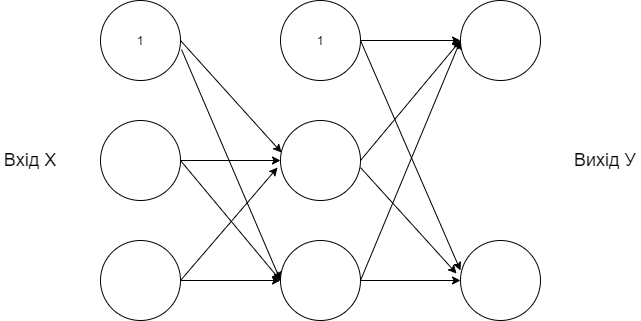
\includegraphics[width=0.82\textwidth]{images/image16.png}\caption{Ілюстрація з вихідної роботи (image16)}\label{fig:image16}\end{figure}
Одними із ключовими характеристиками багатошаровому перцептроні є використання нелінійної функції активації, як правило сигмоїдної. Також у ньому як вже було сказано число шарів, які навчають, більше одного. У загальних випадках використовують не більше трьох.

Сигнали, що одержує модель можуть бути інтерпретовані у десяткових числах. Після цього бажано провести нормалізацію даних значень. Це потрібно робити, оскільки функція активації є сигмоїдальною і приймає значення від 0 до 1.

Навчання багатошарового перцептрону проводиться до стабілізації коефіцієнтів при навчанні або зупиняється не дійшовши кінця навчання, щоб уникнути перенавчання.

\section{Випадковий ліс}
Алгоритм машинного навчання, який називається випадковий ліс \cite{ref7} - це своєрідний оцінювач, який підходить до ряду класифікуючих дерев рішень на різних гілках набору даних і використовує усереднення для підвищення точності прогнозування та контролю над вхідною інформацією.

В основі алгоритм випадкового лісу (Рисунок 5. 4) лежать так звані дерева рішень, за допомогою яких відбувається обробка вхідної інформації . У машинному навчанні дерева рішень - це певний метод для обчислення значень та параметрів моделі у прогнозуванні. Дану назву вони отримали, тому що прийняття та вихідний результат будується по гілкам, таким чином створюється ніби дерево де кожна гілка відповідає на питання "якщо ... тоді ..." - подібно до гілок дерева.

Якщо ми уявимо, що ми почнемо з певної вибірки, для якої ми хочемо передбачити клас чи побудувати регресійну модель, то потрібно починати з низу гілки і йти по рішенням вгору , щоб отримати відповідь, поки не дійдемо до першої розгалуженої гілки. Це розгалуження можна вважати як особливість даного методу машинного навчання, і питання в тому де вона з’явиться. Тепер йде послідовне прийняття рішень, щодо того чи йти далі чи обрати іншу гілку для обробки рішень. Це відбувається до тих пір поки не приймається рішення про перехід на наступну гілку, або повторити процес знову, тим самим покращити результати. Ця кінцева точка називається аркушем, і в деревах рішень представлений кінцевий результат: передбачуваний клас або значення.

\begin{figure}[H]\centering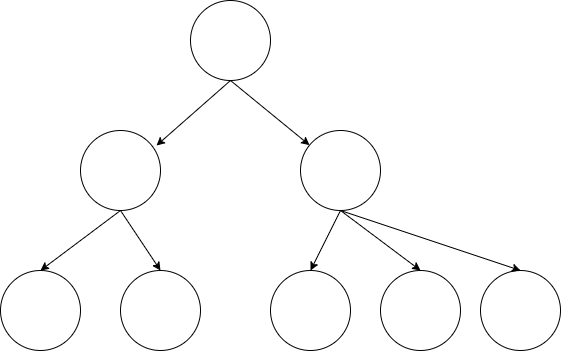
\includegraphics[width=0.82\textwidth]{images/image17.png}\caption{Ілюстрація з вихідної роботи (image17)}\label{fig:image17}\end{figure}
\chapterConclusion
Була описана проблема, що з’являється у випадку використання неповних супутникових знімків, як вхідних даних у модель, що дає безхмарний супутниковий знімок. Зроблений огляд відомого алгоритму color transfer перенесення колірного стилю та описані його недоліки для застосування супутникових знімків. Було оглянуто алгоритми машинного навчання як можливе вирішення проблеми відновлення супутникових даних.
\begin{table}[H]\centering\scriptsize\caption{Класифікація каналів Sentinel-2}\label{tab:source2}\begin{tabular}{|p{0.34\textwidth}|p{0.56\textwidth}|}\hline
Канал & Назва каналу\\\hline
1 & Coastal aerosol\\\hline
2 & Blue\\\hline
3 & Green\\\hline
4 & Red\\\hline
5,6,7 & Vegetati\allowbreak{}on red e\allowbreak{}dge\\\hline
8 & NIR\\\hline
8А & Narrow NIR\\\hline
9 & Water vapour\\\hline
10 & SWIR – Cirrus\\\hline
11,12 & SWIR\\\hline
\end{tabular}\end{table}
\begin{table}[H]\centering\scriptsize\caption{Класифікація об’єктів маски}\label{tab:source3}\begin{tabular}{|p{0.34\textwidth}|p{0.56\textwidth}|}\hline
Значення & Клас\\\hline
0 & Немає інформації\\\hline
1 & Дефектні об’єкти\\\hline
2 & Область \allowbreak{}темних п\allowbreak{}ікселів\\\hline
3 & Тінь хмар\\\hline
4 & Рослинність\\\hline
5 & Не рослинність\\\hline
6 & Вода\\\hline
7 & Не класифіковано\\\hline
8 & Хмара се\allowbreak{}редньої \allowbreak{}прозорос\allowbreak{}ті\\\hline
9 & Не прозорі хмари\\\hline
10 & Прозорі хмари\\\hline
11 & Сніг\\\hline
\end{tabular}\end{table}

\begin{figure}[H]\centering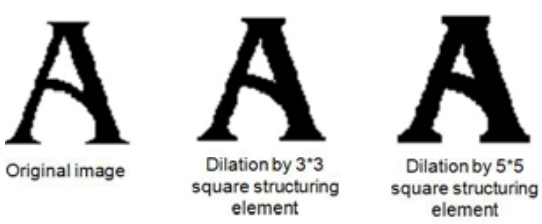
\includegraphics[width=0.7\textwidth]{images/image6.png}\caption{Формула оператора розширення з вихідного документа}\label{fig:dilation-formula}\end{figure}
